\begin{figure}
\centering
\begin{tabular}{lc}
    \hskip0.05cm 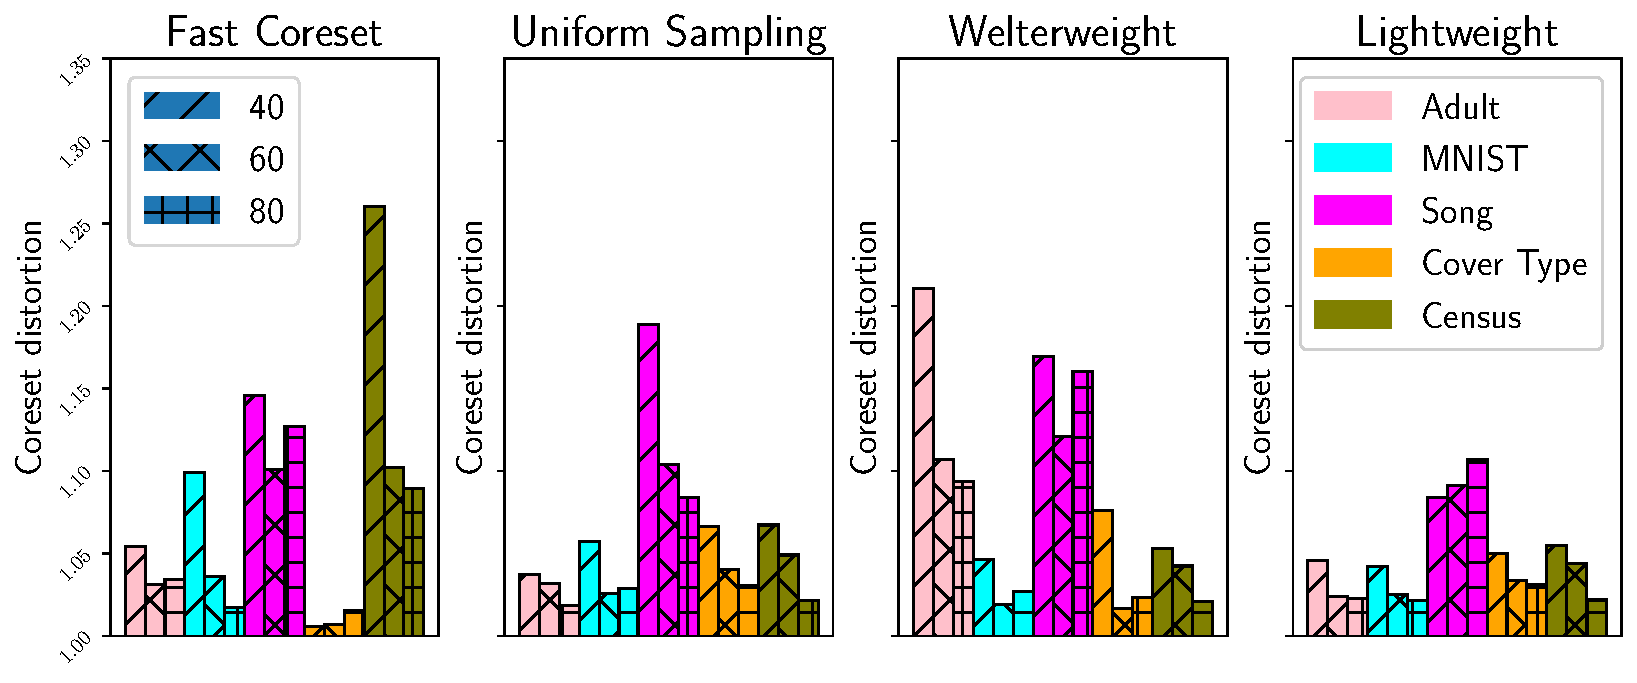
\includegraphics[width=.95\linewidth]{images/distortion_real_data} \\
    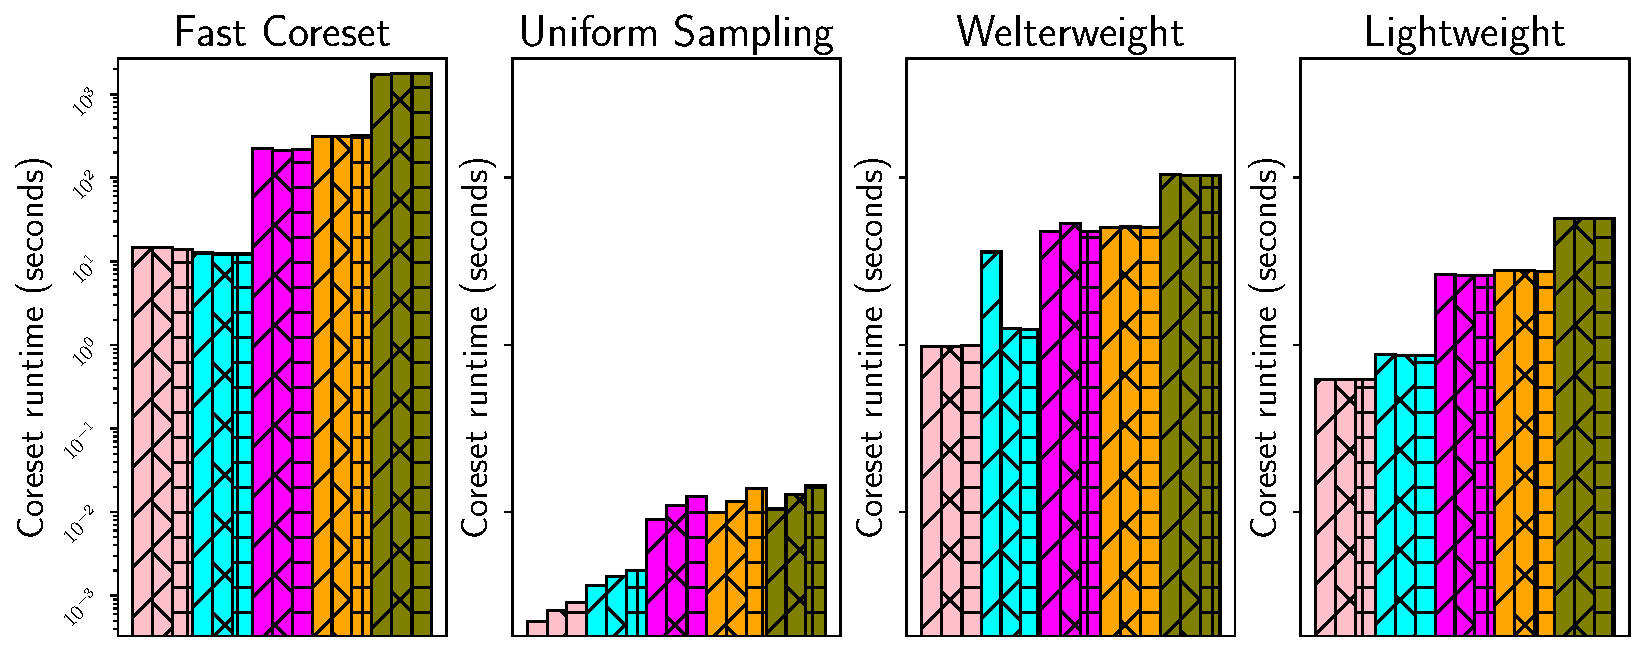
\includegraphics[width=.955\linewidth]{images/runtime_real_data}
\end{tabular}
\caption{\emph{Top}: The effect of the $m$-scalar on the distortion metric for real-world datasets.  \emph{Bottom}: The effect of the $m$-scalar on the
algorithm runtime for real-world datasets. All values are the mean over 5 runs and y-axis is log-scale. The three bars represent samples of size $m=40k, 60k,
80k$.}
\label{fig:coreset_size_on_quality}
\end{figure}
